\section{A Control Function Approach}
\label{sec:controlfun}
% A selection model relies on the errors follow a known distribution, and identification is disrupted when the errors follow some other distribution.
% A control function approach avoids these assumptions, which are dubious in practice, by instead relying on instrument.\footnote{
%     This section does not improve on the control function approach, instead only noting its utility to solve the identification problem of CM in a natural experiment setting.
% }
If your goal is to estimate CM effects, and you could control for unobserved selection terms $U_{0,i}, U_{1,i}$, then you would.
This ideal example would yield unbiased estimates.
% Alas, $U_i$ is by definition unobserved.
The control function method takes this insight seriously, providing conditions to model the unobserved $\left(U_{0,i}, U_{1,i}\right)$, and then control for it.\footnote{
    This section does not improve on the control function approach, instead only noting its utility to solve the identification problem of CM in a natural experiment setting.
}

Write $K_i$ for the expected values in predicting the mediator with observed data $Z_i, \vec X_i$.
%Then take the two components of $K_i$ into $K_{0 ,i}, K_{1,i}$, corresponding to whether $i$ refuses or takes the mediator, respectively.
\begin{align*}
    K_i &= D_i - \Egiven{D_i}{Z_i, \vec X_i}
    %, \\
    %K_i &= F_D \left( \bar D_i \mid Z_i, \vec X_i^{\text{IV}}, \vec X_i^- \right)
    %K_{0,i} &= (1 - D_i) K_i, \;\;\; K_{1,i} = D_i K_i.
\end{align*}
Additionally, suppose the vector of control variables $\vec X_i$ has at least two entries;
denote $\vec X_i^{\text{IV}}$ as one entry in the vector, and $\vec X_i^-$ as the remaining rows.
\begin{definition}
    \label{dfn:controlfun-assumptions}
    Control function assumptions.
    \begin{align}
        \label{eqn:firststage-monotonicity}
        &\Probgiven{ D_i(1) \geq D_i(0) }{\vec X_i} = 1 \\
        \label{eqn:controlfun-ident}
        &D_i \indep Y_i(.,.) \; \Big| \; \vec X_i^-, K_i \\
        \label{eqn:controlfun-iv}
        &\vec X_i^{\text{IV}} \textnormal{ satisfies }
        \partialdiff{\vec X_i^{\text{IV}}}\left[
            \mu_1(\vec X_i) - \mu_0(\vec X_i)\right] = 0
            < \partialdiff{\vec X_i^{\text{IV}}}\Egiven{D_i(z')}{\vec X_i},
            \textnormal{ for } z' = 0, 1.
    \end{align}
\end{definition}
Assumption \ref{dfn:controlfun-assumptions}\eqref{eqn:firststage-monotonicity} is the (conditional) monotonicity assumption \citep{imbens1994identification}, which is untestable but acceptable in many empirical applications.
Assumption \ref{dfn:controlfun-assumptions}\eqref{eqn:controlfun-ident} is the control function assumption, assuming that first-stage unobserved heterogeneity explains second-stage selection into $D_i$.
Assumption \ref{dfn:controlfun-assumptions}\eqref{eqn:controlfun-iv} is assuming that an instrument exists, which satisfies an exclusion restriction (i.e., not impacting mediator gains $\mu_1-\mu_0$), and has a non-zero influence on the mediator (i.e., strong first-stage).
The exclusion restriction is untestable, and must be guided by domain-specific knowledge; strength of the first-stage is testable, and must be justified with data by methods common in the instrumental variables literature.

%Here, $K_i$ is equal to the conditional cumulative density function of $D_i$, $\Probgiven{D_i \leq d'}{Z_i, \vec X_i^{\text{IV}}, \vec X_i^-}$ for $d' = 0,1$.
%Thus, $\left( K_{0 ,i}, K_{1,i}\right)$ serves as the control function in this setting.
$K_{i}$ serves as a control function in this setting.
\begin{theorem}
    \label{thm:controlfun}
    If \ref{dfn:controlfun-assumptions}\eqref{eqn:firststage-monotonicity} and \ref{dfn:controlfun-assumptions}\eqref{eqn:controlfun-iv} hold, then the mean potential differences
    (and thus CM effects)
    are identified by a control function approach.
    For each $z', d' = 0,1$,
    % \begin{align*}
    %     \Egiven{Y_i}{Z_i = 1, D_i = d', \vec X_i^-, K_{d',i}}
    %     - \Egiven{Y_i}{Z_i = 0, D_i = d', \vec X_i^-, K_{d',i}} 
    %     &= \Egiven{Y_i(1, d') - Y_i(0, d')}{\vec X_i^-} \\
    %     \Egiven{Y_i}{Z_i = z', D_i = 1, \vec X_i^-, K_{1,i}}
    %     - \Egiven{Y_i}{Z_i = z', D_i = 0, \vec X_i^-, K_{0,i}} 
    %     &= \Egiven{Y_i(z', 1) - Y_i(z', 0)}{\vec X_i^-}.
    % \end{align*}
    \begin{align*}
        \Egiven{Y_i}{Z_i = 1, D_i = d', \vec X_i^-, K_{i}}
        - \Egiven{Y_i}{Z_i = 0, D_i = d', \vec X_i^-, K_{i}} 
        &= \Egiven{Y_i(1, d') - Y_i(0, d')}{\vec X_i^-} \\
        \Egiven{Y_i}{Z_i = z', D_i = 1, \vec X_i^-, K_{i}}
        - \Egiven{Y_i}{Z_i = z', D_i = 0, \vec X_i^-, K_{i}} 
        &= \Egiven{Y_i(z', 1) - Y_i(z', 0)}{\vec X_i^-}.
    \end{align*}
\end{theorem}
\begin{proof}
    Special case of \citet[Theorem~1]{florens2008identification}, \citet[Theorem~3]{imbens2009identification}.
    %; see \autoref{appendix:controlfun-proof}.
\end{proof}

Assumption \ref{dfn:controlfun-assumptions}\eqref{eqn:firststage-monotonicity} guarantees that mediator can be represented by a selection model \citep{vytlacil2002independence}, $D_i(.) = \indicator{\bar\mu(.,;\vec X_i) \geq K_i}$ for some function $\bar\mu$.
Assumption \ref{dfn:controlfun-assumptions}\eqref{eqn:controlfun-ident} connects the first- and second-stage for identification.
Assumption \ref{dfn:controlfun-assumptions}\eqref{eqn:controlfun-iv} separately identifies the control function to identify the second-stage model.
The approach exploits the fact that the bias terms, coming from correlated the errors in \autoref{sec:regression}, can be estimated in a first-stage regression and included as controls in the second-stage.

If the underlying selection model had been a Roy model, the control function approach captures the unobserved benefits to taking mediator (independent of observed controls), and thus driving take-up of the mediator.
In this case, $K_i = U_{C,i} - (U_{1,i} - U_{0,i})$, so the independence result is simple.
By incorporating the control function from the first-stage model, the approach adjusts for the unobserved confounding from unobserved gains, $U_{1,i} - U_{0,i}$.
By contrast, assuming the mediator was ignorable would have been assuming that there are no unobserved benefits to the mediator take-up, so that there is no bias in the second-stage to account for.

The instrument is key to avoid distributional assumptions on the unobserved errors terms.
In the Roy model, the exclusion restriction can be satisfied in one key way: having an instrument for cost of mediator take up $\mu_C$.
If the instrument $\vec X_i^{\text{IV}}$ enters the cost function $\mu_C$, and not the benefits function $\mu$, then it satisfies the exclusion restriction.
In an applied world, $\vec X_i^{\text{IV}}$ can be data that explain cost differences in taking $D_i$, unrelated to other demographic information.
If a researcher is looking into higher education as a proposed mediator, then data which explains different costs of attending university (unrelated to education gains) can serve this role.
This is the logic behind the \cite{card1993using} distance-instrument, and can be extended to a CM setting with education as the mediator.

%\textbf{Senan note:} Needs a step involving re-weighting to the D(z) compliers in the LAIE estimation.
% This is done by estimating the second-stage with Abadie (2003) re-weighting.

\subsection{Estimation}
In practice, the approach relies on estimating the control function $K_i$, then including this in the second-stage as a control, and accounting for the estimation error for these in the standard errors.
These reliances come with major concerns.
First, it is imperative that the control function is estimated correctly, so it is necessary to employ a non-parametric approach to estimate the first-stage.
Second, the error terms enters the second-stage \eqref{eqn:parametric-secondstage} linearly, but is an unknown function (possibly non-linear) of the control function; thus, the second-stage must be estimated semi-parametrically.\footnote{
    In practice this can be done by adding a polynomial for the estimated control function into the outcome regression, or a splines approach, etc. 
}
Lastly, the standard errors must account for estimation uncertainty in the above two non-parametric steps.

These concerns are worth noting, because non-parametric regression is computationally demanding, and requires large samples for estimator convergence. 
Furthermore, these are estimated in two steps, so that the concerns are of greater importance.
Otherwise, small sample bias properties could even dominate the bias terms identified in \autoref{thm:selection-bias}.\footnote{
    See \cite[Section~6]{imbens2009identification} for a full discussion of the asymptotic theory of a control function estimator.
}
It is beyond the scope of this paper to develop the optimal procedure here, but these concerns are important.
% Senan note: future direction?  Needs consistency results, too.
% Might need a competent econometrician coauthor, as Senan is not....
For applied research aiming to estimate CM effects, the control function method is only appropriate in extremely large sample sizes, such as applications using administrative sources or biobanks.

With these concerns in mind, I propose the following method to estimate CM effects with a control function approach:
\begin{enumerate}
    \item Estimate the first-stage, $\Egiven{D_i}{Z_i, \vec X_i^{\text{IV}}, \vec X_i^-}$ with a non-parametric estimator (e.g., a probability forest, or fully interacted OLS specification).
    \item Calculate estimates of the control function:
    \begin{align*}
        \hat K_i &= D_i - \hat{\mathbb E} \left[D_i \middle\vert Z_i, \vec X_i^{\text{IV}}, \vec X_i^- \right].
        %, \\
        %\hat K_{0,i} &= (1 - D_i) \hat K_i, \;\;\;
        %    \hat K_{1,i} = D_i \hat K_i.
    \end{align*}
    \item Estimate the second-stage with OLS (including an interaction term between $Z_i$ and $D_i$), and a semi-parametric regressor of the control function.
    \[ \mathbb{E} \left[Y_i \middle\vert Z_i, D_i, \vec X_i^-, \hat K_{0,i}, \hat K_{i}\right]
    = \beta D_i + \gamma Z_i + \delta Z_i D_i + l\left( \hat K_{i}\right) \]
    %$l_0(.), l_1(.)$ are
    $l(.)$ is a nuisance function with unknown form, so can be approximated with a semi-parametric spline specification, for example.
    \item Calculate the ADE and AIE estimates from the first and second-stages.
    \begin{align*}
        \hat{\text{ADE}} &= \; \E{
            \hat{\mathbb{E}} \left[ Y_i \middle\vert Z_i = 1, D_i, \vec X_i^-, \hat K_i \right]
            - \hat{\mathbb{E}} \left[ Y_i \middle\vert Z_i = 0, D_i, \vec X_i^-, \hat K_i \right]} \\
        \hat{\text{AIE}} &= \; \mathbb E \left[ \begin{aligned} &\left(
            \hat{\mathbb{E}} \left[D_i \middle\vert Z_i = 1, \vec X_i^{\text{IV}}, \vec X_i^-\right]
            - \hat{\mathbb{E}} \left[D_i \middle\vert Z_i = 1, \vec X_i^{\text{IV}}, \vec X_i^-\right] \right) \\
            &\times \left(
                \hat{\mathbb{E}} \left[ Y_i \middle\vert Z_i, D_i = 1, \vec X_i^-, \hat K_i \right]
            - \hat{\mathbb{E}} \left[ Y_i \middle\vert Z_i, D_i = 0, \vec X_i^-, \hat K_i \right]
            \right) \end{aligned} \right]
    \end{align*}
    %\item Estimate the second-stage with weighted-least squares, including a control function with (estimated) $\kappa$-weights \citep{abadie2003semiparametric}.
    %\begin{align*}
    %    \hat\kappa_i &= \; 1 - \frac{(1 - Z_i)D_i}{
    %        1 - \hat\Pr\left(Z_i = 1 \middle\vert \vec X_i^-, \vec X_i^{\text{IV}}\right)} -
    %        \frac{Z_i (1 - D_i)}{
    %        \hat\Pr\left(Z_i = 1 \middle\vert \vec X_i^-, \vec X_i^{\text{IV}}\right)} \\
    %    \mathbb{E} \left[ \hat\kappa_i Y_i \middle\vert Z_i, D_i, \vec X_i^-, \hat K_i \right]
    %        &= \beta D_i + \gamma Z_i + \delta Z_i D_i + l\left( \hat K_i \right)
    %\end{align*}
    %Estimate the AIE from this second-stage.
    %\begin{align*}
    %    \hat{\text{AIE}} &= \; \mathbb E \left[ \begin{aligned} &\left(
    %        \hat{\mathbb{E}} \left[D_i \middle\vert Z_i = 1, \vec X_i^{\text{IV}}, \vec X_i^-\right]
    %        - \hat{\mathbb{E}} \left[D_i \middle\vert Z_i = 1, \vec X_i^{\text{IV}}, \vec X_i^-\right] \right) \\
    %        &\times \left(
    %            \hat{\mathbb{E}} \left[ \hat\kappa_i Y_i \middle\vert Z_i, D_i = 1, \vec X_i^-, \hat K_i \right]
    %        - \hat{\mathbb{E}} \left[ \hat\kappa_i Y_i \middle\vert Z_i, D_i = 0, \vec X_i^-, \hat K_i \right]
    %        \right) \end{aligned} \right]
    %    \end{align*}
    \item Bootstrap across the previous steps, to calculate standard errors for the respective ADE and AIE estimates.
\end{enumerate}

\subsection{Simulation Evidence}
The following simulation gives an example to show how this method works in practice.
Suppose data observed to the researcher $Z_i, D_i, Y_i, \vec X_i$ are drawn from the following data generating processes, for $i = 1, \hdots, N$.
\begin{align*}
    Z_i \sim \text{Binom}\left(0.5 \right),
    \;\; \vec X_i^- \sim N(4, 1),
    \;\; \vec X_i^{\text{IV}} \sim \text{Binom}\left( 0.5 \right), \\
    \left( U_{0,i}, U_{1,i} \right) \sim
    \text{BivariateNormal}\left( 0, 0, \sigma_0, \sigma_1, \rho \right),
    \;\; U_{C,i} \sim N(0, 0.5).
\end{align*}
$N = 10,000$ allows the large sample properties of the approach to operate; indeed, smaller sample sizes may not.

Suppose each $i$ chooses to take mediator $D_i$ by a Roy model, with following mean definitions for each $z', d' = 0, 1$.
\begin{align*}
    D_i(z') = \indicator{Y_i(z', 1) - Y_i(z', 0) \geq C_i},  \\
    \mu_{d'}\left(z' ; \vec X_i \right) = \vec X_i^- + \left( z' + d' + z' d' \right),
    \;\; \mu_{C}\left(z' ; \vec X_i \right) = 3z' + \vec X_i^- - \vec X_i^{\text{IV}}.
\end{align*}
Following \autoref{sec:applied}, these data have the following first and second-stage equations:
\begin{align*}
    D_i &= \indicator{-3Z_i - \vec X_i^{\text{IV}} + \vec X_i^-
        \geq U_{C,i} - \Big( U_{1,i} - U_{0,i} \Big)},  \\
    Y_i &= Z_i + D_i + Z_i D_i + \vec X_i^-
        + \left( 1 - D_i \right) U_{0,i} + D_i U_{1,i}.
\end{align*}
$Z_i$ has an effect on outcome $Y_i$, and it operates partially through mediator $D_i$.
Outcome mean $\mu_{D_i}(Z_i;.)$ contains an interaction term, $Z_i D_i$, so while both $Z_i$ and $D_i$ have constant partial effects, the ATE depends on how many $i$ choose to take the mediator.
In this simulation $\Prob{D_i = 1} = 0.437$, and $65.29\%$ of the sample are mediator compliers (where $D_i(1)=1$ and $D_i(0) = 0$).
This gives an ATE ($Z\to Y$) value of 2.58, ADE 1.44, and AIE 1.13, respectively.\footnote{
    Note that ATE $=$ ADE $+$ AIE, in this setting.
    $\Prob{Z_i=1} = 0.5$ ensures this equality, but is not guaranteed in general.
}

After $Z_i$ is assigned, $i$ chooses to take mediator $D_i$ by considering the costs and benefits --- which vary based on $Z_i$, demographic controls $\vec X_i$, and the (non-degenerate) unobserved error terms $U_{i,0}, U_{1,i}$.
As a result, sequential ignorability does not hold; the mediator is not conditionally ignorable.
Thus, a standard OLS (selection-on-observables) approach to CM does not give an estimate for how much of the $Z \to Y$ ATE goes through mediator $D$.
Instead, the OLS approach gives biased inference.

\begin{figure}[h!]
    \caption{Simulated Distribution of CM Effect Estimates.}
    \begin{subfigure}[c]{0.475\textwidth}
        \centering
        \caption{ADE.}
        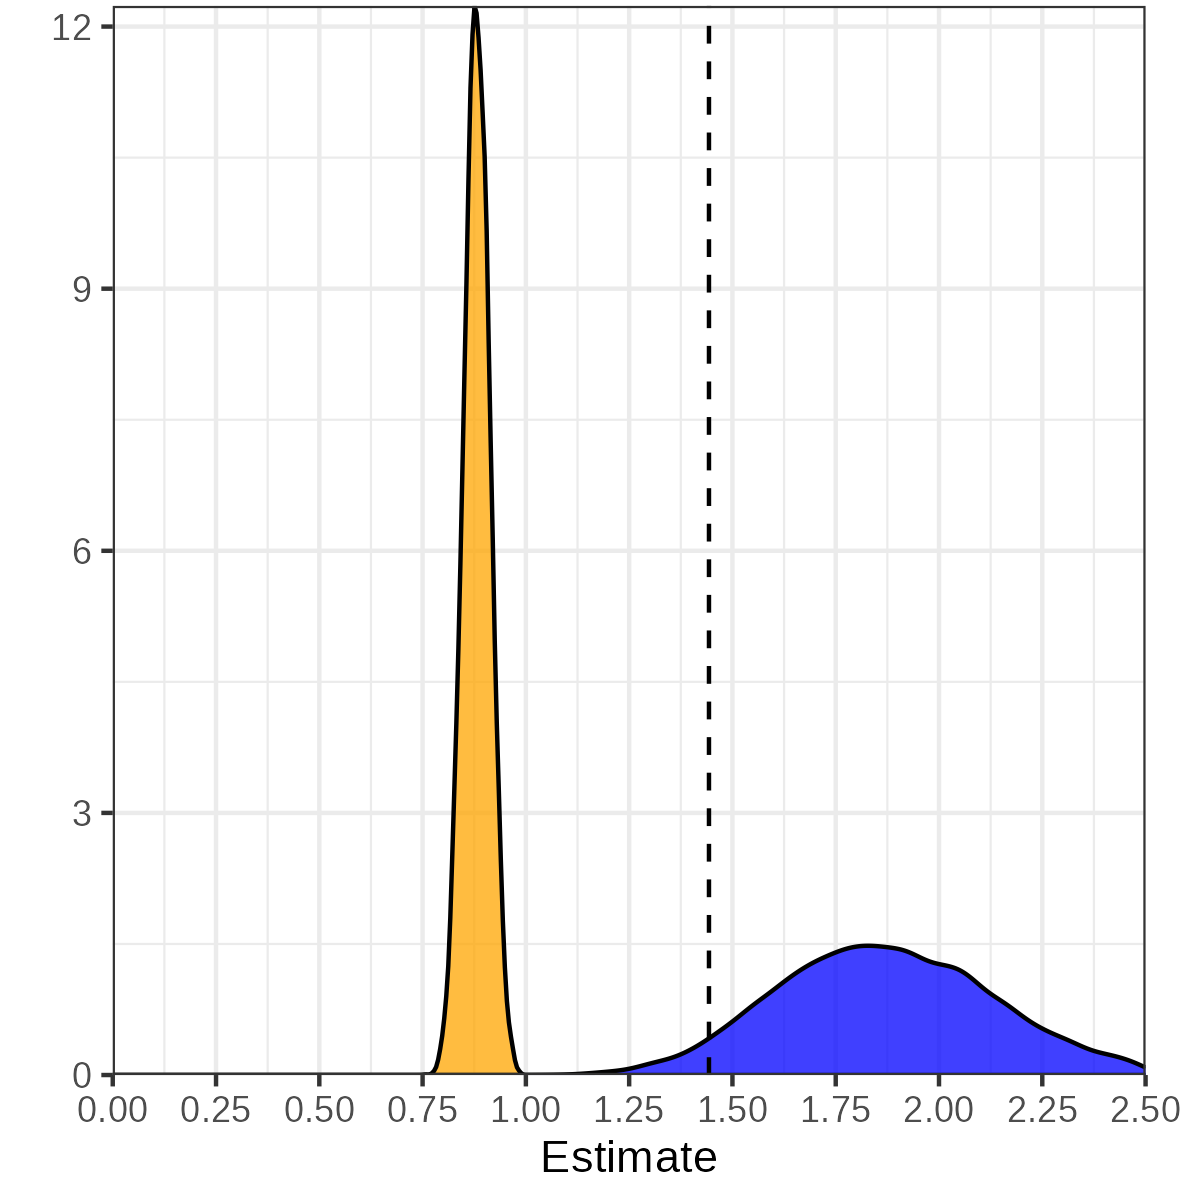
\includegraphics[width=\textwidth]{
            ../programs/simulations/sim-output/direct-boot.png}
    \end{subfigure}
    \begin{subfigure}[c]{0.475\textwidth}
        \centering
        \caption{AIE.}
        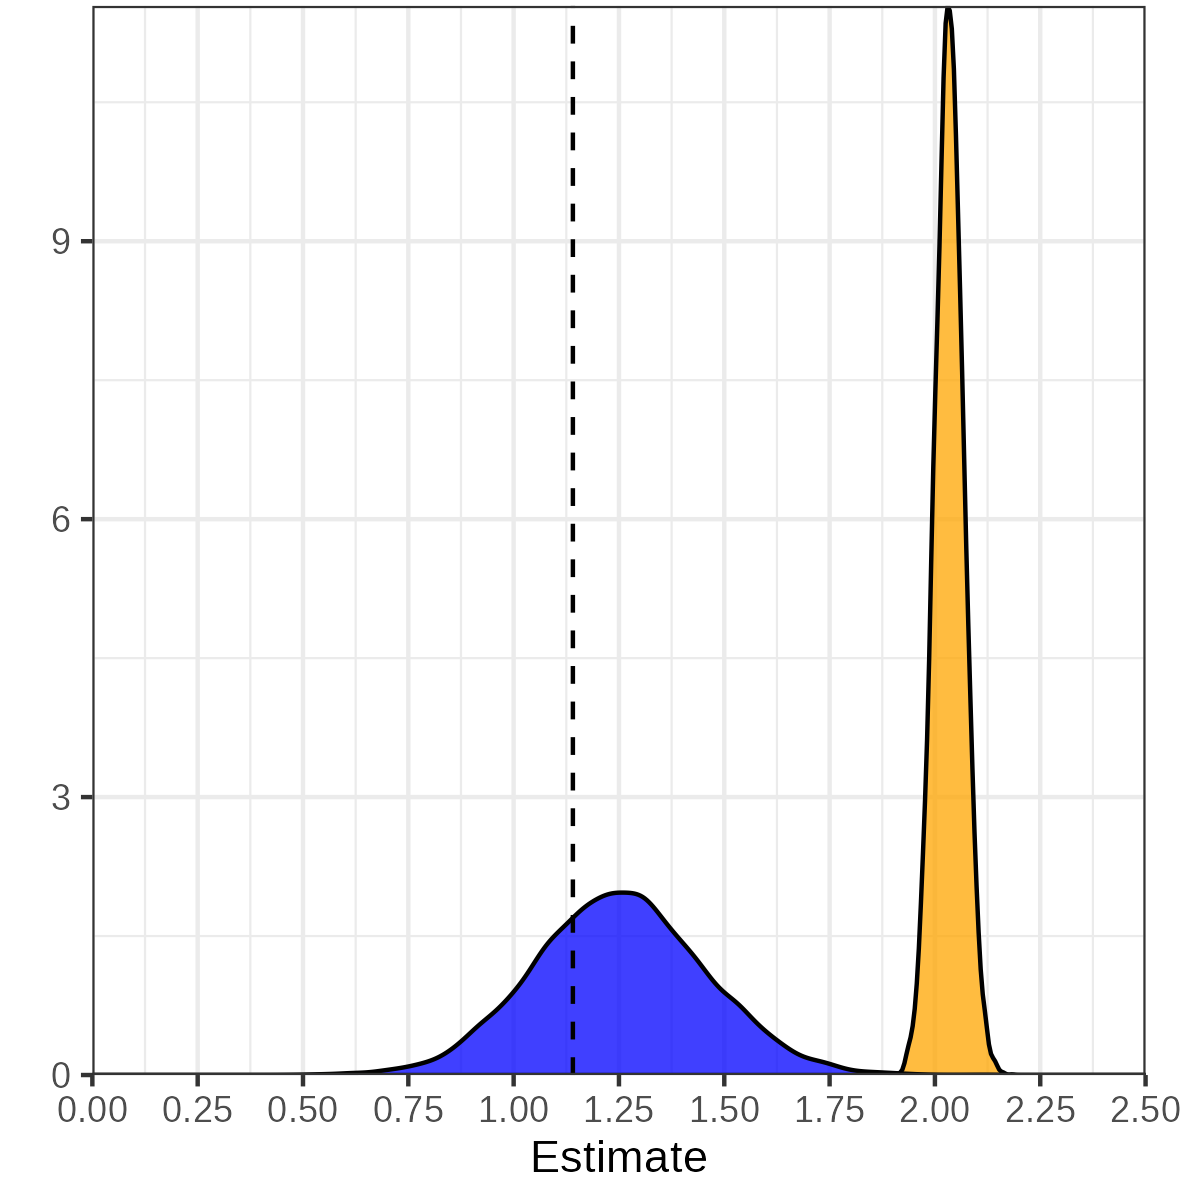
\includegraphics[width=\textwidth]{
            ../programs/simulations/sim-output/indirect-boot.png}
    \end{subfigure}
    \label{fig:cm-boot-dist}
    \justify
    \footnotesize    
    \textbf{Note:}
    These figures show the empirical density of point estimates, for 10,000 replications of the data generating process described above.
    The black dashed line is the true value;
    orange is the distribution of na\"ive OLS estimates, and blue the control function approach.
\end{figure}

The bias in OLS estimates comes from the unobserved error terms being related.
\autoref{fig:cm-boot-dist} shows the distribution of bootstrapped point estimates in this simulation, showing OLS against the control function approach.
The OLS approach implicitly assumes that the mediator is ignorable (when it is not), so its point estimates under and over-estimate the true ADE and AIE, respectively.
The distance between the OLS estimates and the true values are the underlying bias terms derived in \autoref{thm:selection-bias}.
In this data generating process, the OLS confidence interval do not overlap the true values for any standard level of significance.
The control function approach exhibits bias, though the 95\% confidence intervals cover the truth.

\begin{figure}[h!]
    \caption{Point Estimates of CM Effects, OLS versus Control Function, varying $\rho$ values with $\sigma_0 = 1, \sigma_1 = 2$ fixed.}
    \begin{subfigure}[c]{0.475\textwidth}
        \centering
        \caption{ADE.}
        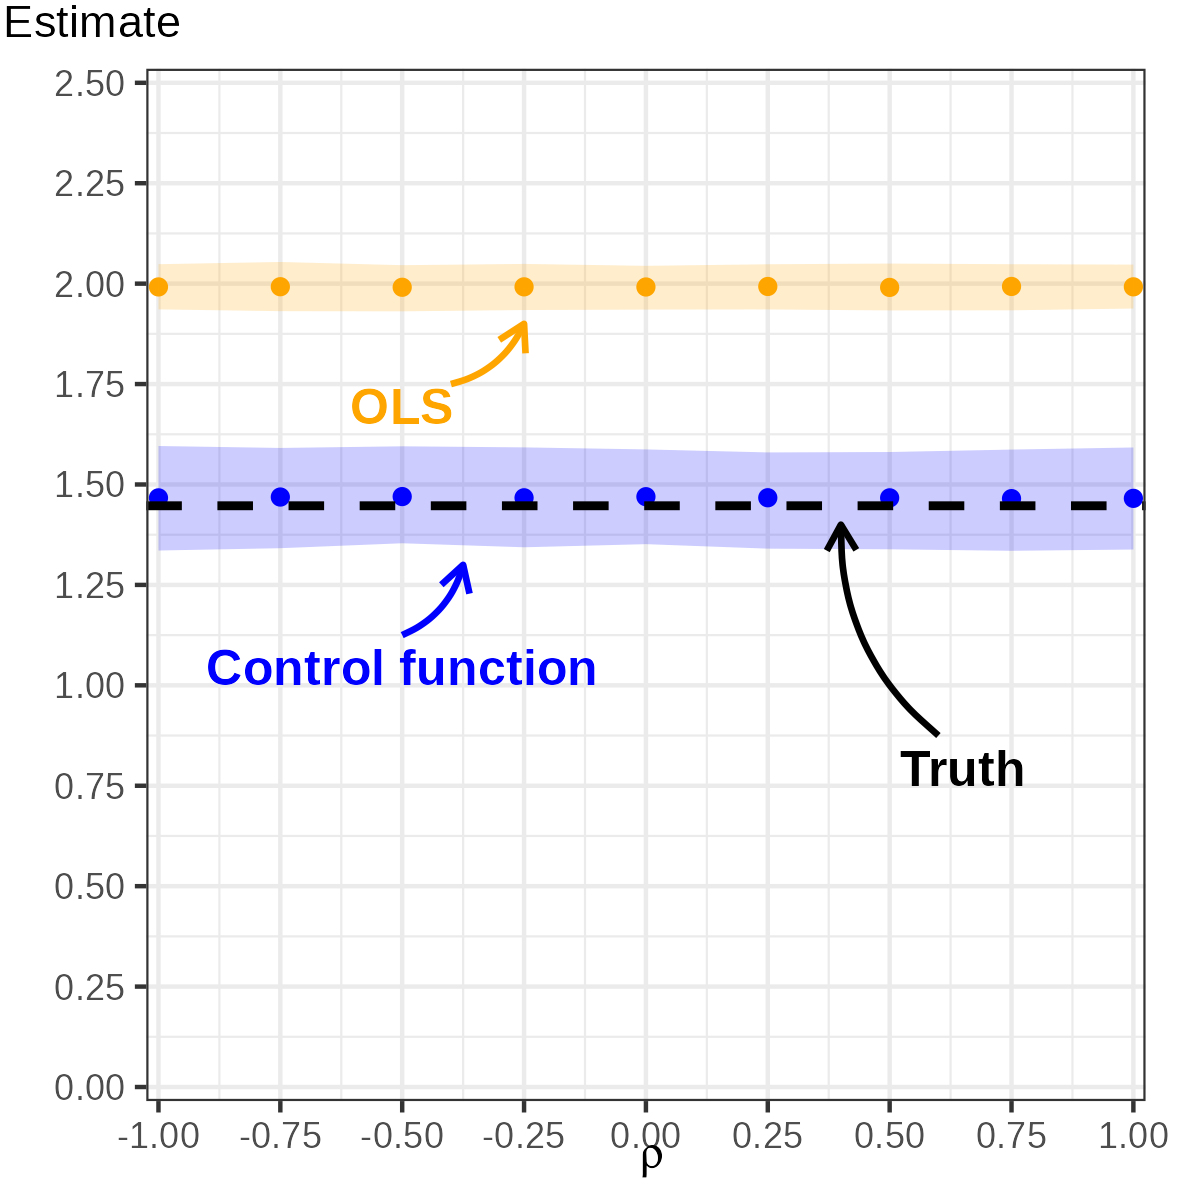
\includegraphics[width=\textwidth]{
            ../programs/simulations/sim-output/rho-directeffect-bias.png}
    \end{subfigure}
    \begin{subfigure}[c]{0.475\textwidth}
        \centering
        \caption{AIE.}
        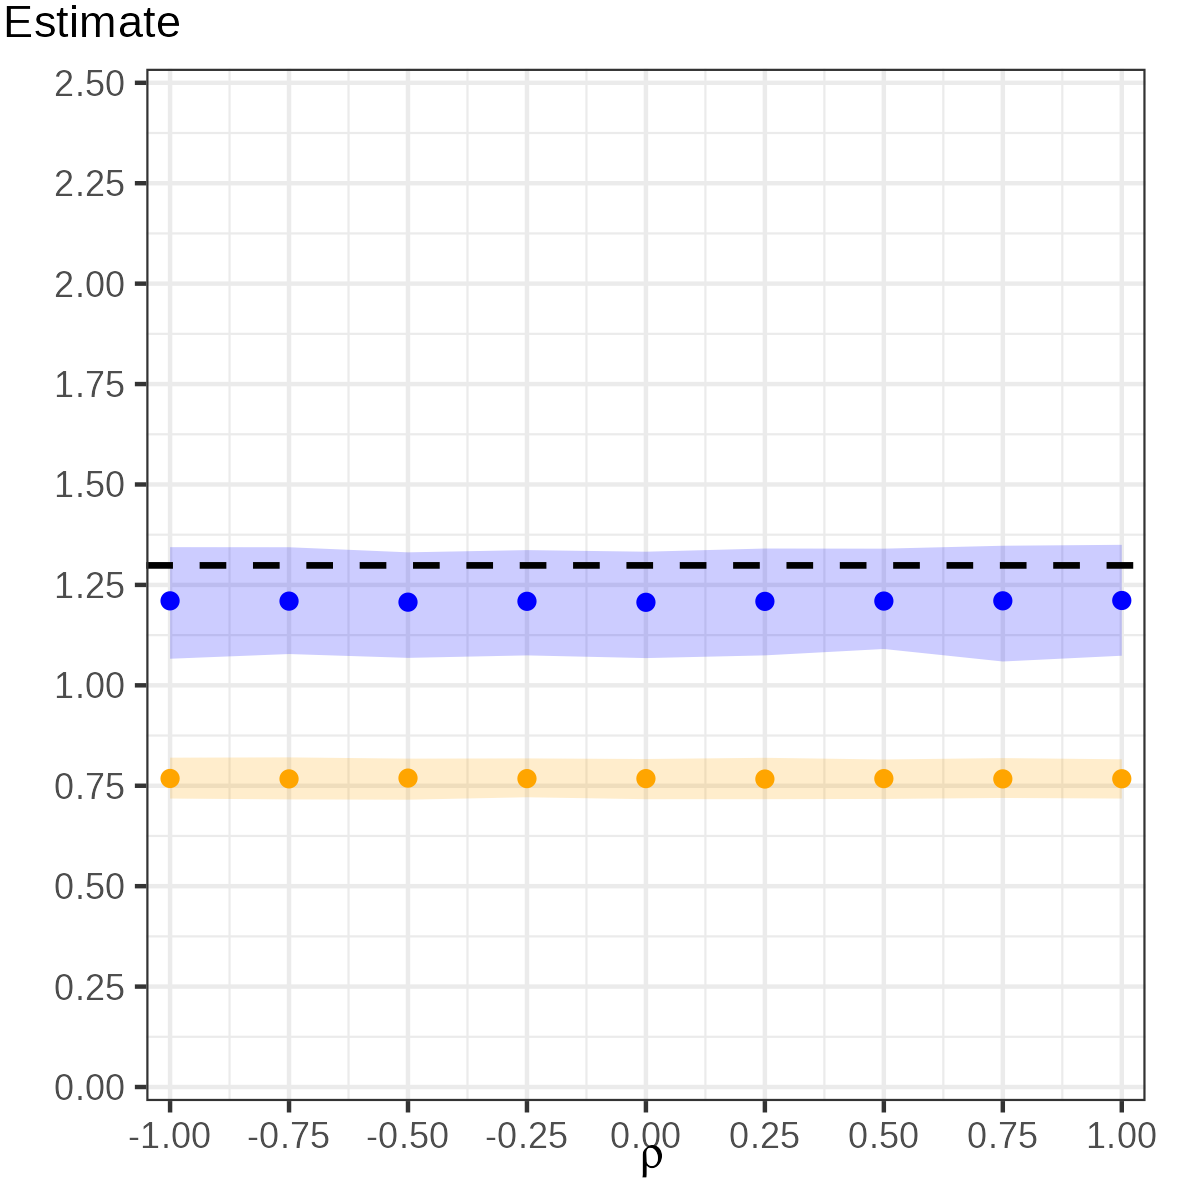
\includegraphics[width=\textwidth]{
            ../programs/simulations/sim-output/rho-indirecteffect-bias.png}
    \end{subfigure}
    \label{fig:rho-bias}
    \justify
    \footnotesize    
    \textbf{Note:}
    These figures show the OLS and control function point estimates of the ADE and AIE, for $N = 10,000$ sample size.
    The black dashed line is the true value, points are points estimates from data simulated with a given $\rho$ value and $\sigma_0 = 1, \sigma_1 = 2$, and shaded regions are the 95\% confidence intervals from 1,000 bootstraps each.
    Orange represents OLS estimates, blue the control function approach.
    The true AIE values vary with $\rho$, because $D_i(Z_i)$ compliers have higher average values of $U_{1,i} - U_{0,i}$ with greater $\rho$ values.
\end{figure}

The error terms determine the bias in OLS estimates of the ADE and AIE, so the bias varies for different values of the error-term parameters $\rho \in [-1, 1]$ and $\sigma_0, \sigma_1 \geq 0$.\footnote{
    Indeed, this setting has error terms following a bivariate normal distribution, so the canonical \cite{heckman1974shadow} selection model would produce the most efficient estimates by maximum likelihood.
    The control function approach avoids this assumption, and bias from breaking it, by relying on an instrument.
}
\autoref{fig:rho-bias} shows control function estimates against estimates calculated by standard OLS, showing 95\% confidence intervals calculated from 1,000 bootstraps.
The point estimates of the control function do not exactly equal the true values, as they are estimates from one simulation (not averages across many simulations, as in \autoref{fig:cm-boot-dist}).
The control function approach improves on OLS estimates by correcting for bias, with confidence regions overlapping the true values.\footnote{
    The code behind this simulation estimates the first-stage with an interacted OLS specification, and splines included for the continuous regressor $\vec X_i^-$.
    The second-stage is an OLS specification, including the control function with a spline specification.
}$^,$\footnote{
    In the appendix, \autoref{fig:sigma-bias} shows the same simulation while varying $\sigma_1$, with fixed $\sigma_0 = 1, \rho = 0.5$.
    The conclusion is the same as for varying the correlation coefficient, $\rho$, in \autoref{fig:rho-bias}.
}
This correction did not come for free: the standard errors are significantly greater in a control function approach than OLS.
Standard errors on the AIE are larger than those for the ADE, because the AIE estimates are first-stage times second-stage estimates, so standard errors account for uncertainty in both estimates multiplied.
%(i.e., the same reasons instrumental variables estimates are less efficient than ideal OLS estimates). 
In this manner, this simulation shows the pros and cons of using the control function approach to estimating CM effects in practice.
